% ------------------------------------------------------------
\section{Calendar Week}
% ------------------------------------------------------------
% --------------------------------------------------- Slide --
\subsection{CW 10+11}
% ------------------------------------------------------------
\begin{frame}
  \frametitle{Review CW 10+11}
	\begin{itemize}
		\item Read papers Weinans1992, Mullender1994 and Lian2010 about bone remodeling algorithms (see attachment to email). Example of a plate representing simplified trabecular bone is shown in all 3 papers with results. We tried to reproduce these results with our own work. \textcolor{green}{Done}
		\item New APDL Script written, based on the one used for exercises provided by Uni Ulm. \textcolor{green}{Done}
		\item A lot of work to get the first results right. But now there is a fair agreement between our results and the results presented in the paper Weinans1992. \textcolor{green}{Done}
	\end{itemize}
\end{frame}

\begin{frame}
  \frametitle{Review CW 10+11 - Reproduction of Literature Results}
	\begin{figure}
		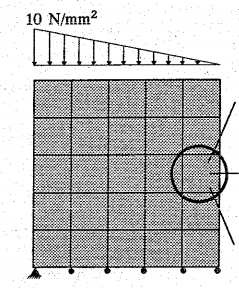
\includegraphics[width=0.3\textwidth]{pictures/2022_CW10+11_1}
	\end{figure}
	\centering Square plate representing "simplified trabecular bone" for study purposes of remodeling algorithm. 
	
	\centering Linear varying load on top edge, fixed support on bottom left corner, frictionless support on bottom edge. 
\end{frame}

\begin{frame}
  \frametitle{Review CW 10+11 - Reproduction of Literature Results}
	\begin{figure}
		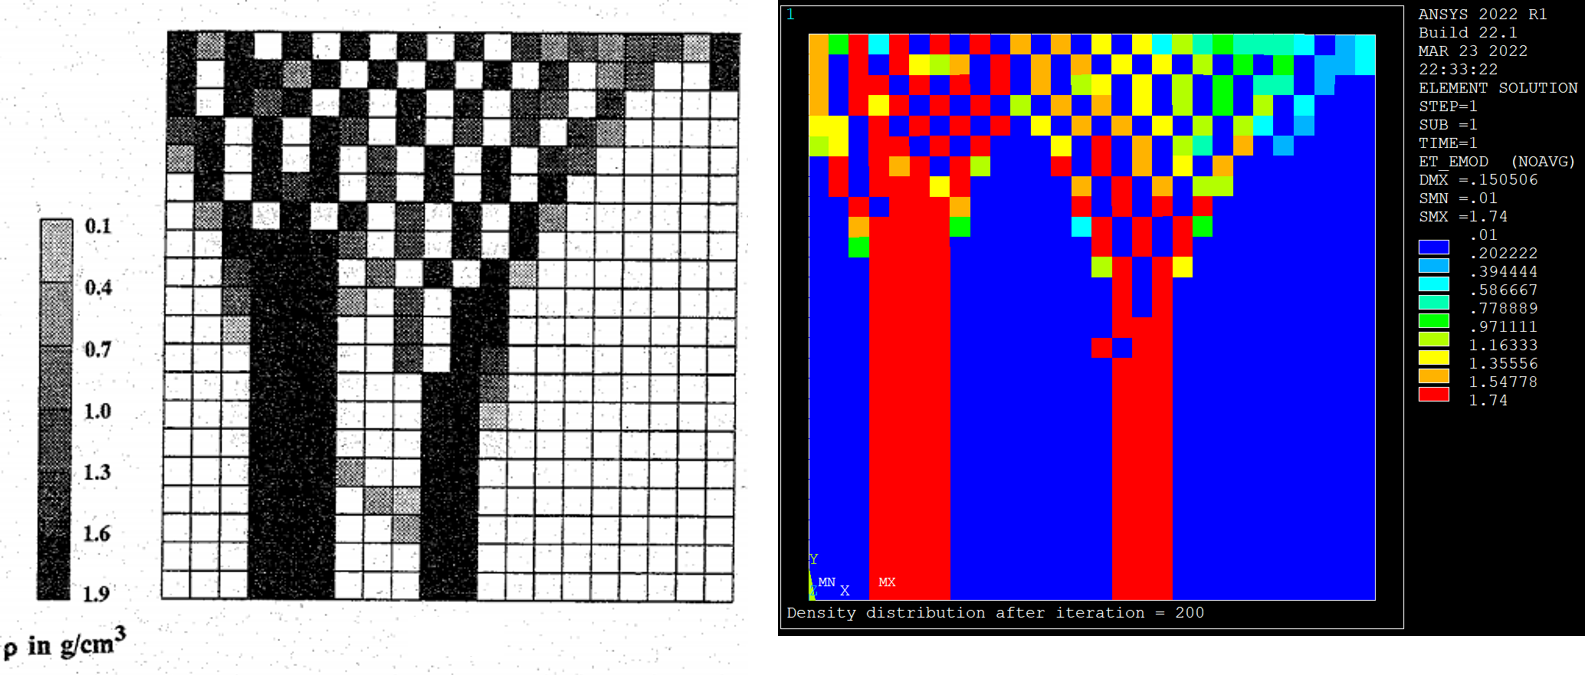
\includegraphics[width=0.9\textwidth]{pictures/2022_CW10+11_2}
	\end{figure}
	\centering Density distribution after remodeling. 
	
	\centering Results presented in the literature (left, from Weinans1992).
	
	\centering Results obtained in this work implementing equivalent algorithm with same parameters and similar mesh as in Weinans1992 (right).
\end{frame}

% ------------------------------------------------------------
% --------------------------------------------------- Slide --
\subsection{CW 12}
% ------------------------------------------------------------
% ------------------------------------------------------------
\begin{frame}
  \frametitle{Outlook CW 12}
	\begin{itemize}
		\item Reproduce bone remodeling algorithm of the other two papers mentioned in the first slide (Mullender1994 and Lian2010), which can be considered as evolution of the Weinans1992 algorithm. This should allow to get rid of the checker-board issue shown in the results of the previous slide.
		\item Further development of own APDL script for bone remodeling. Consider a simplified geometry of bone and implant with a single material.
	\end{itemize}
\end{frame}
% --------------------------------------------------- Slide --

